\documentclass[a4paper]{report}

\usepackage[british]{babel}

\usepackage{listings}
\usepackage{color}

\usepackage{graphicx}
\graphicspath{ {./images/} }

\usepackage{wrapfig}

\definecolor{dkgreen}{rgb}{0,0.6,0}
\definecolor{gray}{rgb}{0.5,0.5,0.5}
\definecolor{mauve}{rgb}{0.58,0,0.82}

\lstset{frame=tb,
  language=C,
  aboveskip=3mm,
  belowskip=3mm,
  showstringspaces=false,
  columns=flexible,
  basicstyle={\small\ttfamily},
  numbers=left,
  numberstyle=\tiny\color{gray},
  keywordstyle=\color{blue},
  commentstyle=\color{dkgreen},
  stringstyle=\color{mauve},
  breaklines=true,
  breakatwhitespace=true,
  tabsize=4
}

\title{A Level Computer Science NEA}
\author{Bailey Harrison}
\date{
	\today\endgraf\bigskip
	Z80 Assembler
}

\begin{document}

\maketitle

\tableofcontents



\chapter{Analysis}

\section{Introduction}

An assembler is a computer program that translates low-level assembly
instructions into raw machine code and data. Unlike compilers and interpreters,
assemblers lack many of the high-level control statements that most programmers
are used to, such as 'if' statements and 'for' loops.

Generally, there is a 1:1 correspondence between assembler opcodes (an acronym
specifying the operation) and machine code instructions (the binary data that a
CPU decodes and executes). Assemblers also support a few other features, notably
labels. A label serves as a placeholder for a memory address, which can be used
to implement variables and functions in a program. In the case of my project, I
am writing an writing an assembler for the Z80 processor architecture.

\bigskip

\begin{wrapfigure}{l}{0.25\textwidth}
    \centering
    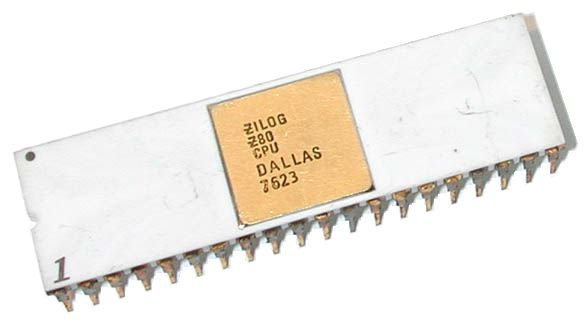
\includegraphics[width=0.25\textwidth]{z80}
\end{wrapfigure}

The Z80 CPU is a microprocessor invented by Zilog in 1975 as their first
product. It was designed as a largely software-compatible extension of the Intel
8080 CPU. Despite the Z80 being originally designed for use in embedded systems,
it gained massive popularity in the desktop market. The Z80 was used in
countless personal computers in the time period, such as the ZX 81, ZX Spectrum,
and Amstrad CPC. Many older game consoles also used this processor, notable the
Nintendo Gameboy and Sega Game Gear. In the modern day, the Zilog Z80 continues
to be used in Texas Instruments' line of TI-83/84 graphing calculators.

\section{Problem}

When programming for older computer systems, you have to take into account the
limited processing power and memory of these systems. Higher-level languages
have a performance overhead and their abstract nature prevents the programmer
from fully taking advantage of the available hardware. Even common "systems"
languages like C and C++ do not allow the programmer to have full control of
memory allocation, register usage, and what particular machine code instructions
are generated.

It is for this reason that retro computer programmers almost exclusively use an
assembly language for development.

\section{System Objectives / Specification}

\subsection{Required}

\begin{enumerate}
	\item Allow assembly of the main 256 Z80 instructions
	\item Second item
\end{enumerate}

\subsection{Optional}

\chapter{Design}

Pls refer to technical solution

\chapter{Technical Solution}

\section{Source Files}

\subsection{main.c}
\lstinputlisting{../src/main.c}
\subsection{symtable.c}
\lstinputlisting{../src/symtable.c}
\subsection{assemble.c}
\lstinputlisting{../src/assemble.c}
\subsection{parseline.c}
\lstinputlisting{../src/parseline.c}
\subsection{util.c}
\lstinputlisting{../src/util.c}

\section{Header Files}

\subsection{symtable.h}
\lstinputlisting{../src/symtable.h}
\subsection{assemble.h}
\lstinputlisting{../src/assemble.h}
\subsection{parseline.h}
\lstinputlisting{../src/parseline.h}
\subsection{util.h}
\lstinputlisting{../src/util.h}



\chapter{Testing}



\chapter{Appraisal}



\end{document}
